\documentclass{standalone}
\usepackage{tikz}
\usetikzlibrary{patterns}
\usetikzlibrary{positioning}
\usetikzlibrary{patterns, positioning}
\usetikzlibrary{shapes.misc}
\usepackage[outline]{contour}
\contourlength{1.5pt} 


\begin{document}
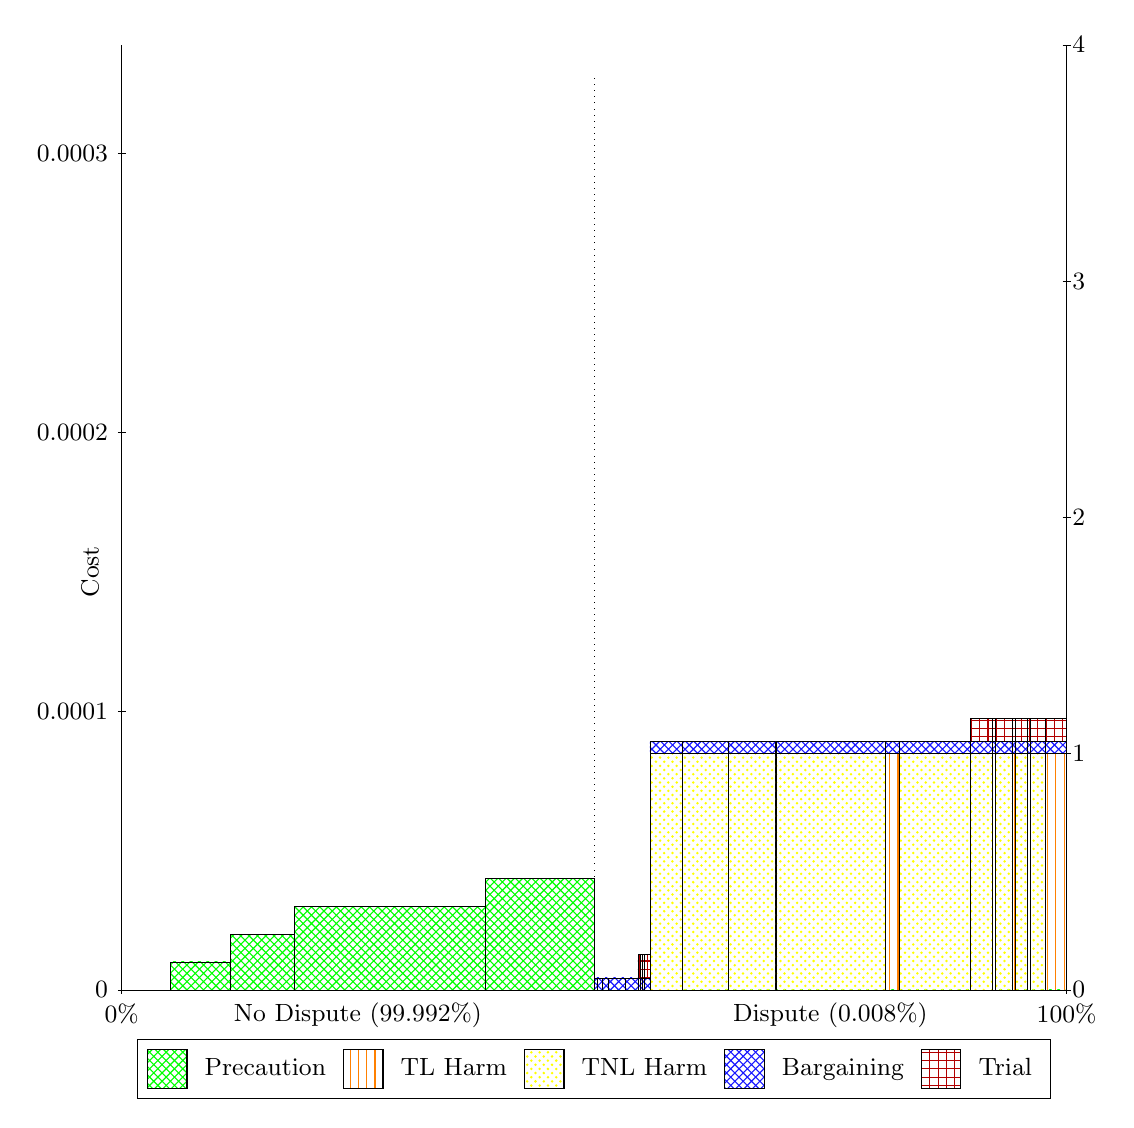
\begin{tikzpicture}
\draw[pattern=crosshatch, pattern color=green,draw=black,very thin] (2.117,2.5) rectangle (2.8801,2.8539);
\draw[pattern=crosshatch, pattern color=green,draw=black,very thin] (2.8801,2.5) rectangle (3.6907,3.2079);
\draw[pattern=crosshatch, pattern color=green,draw=black,very thin] (3.6907,2.5) rectangle (6.1199,3.5618);
\draw[pattern=crosshatch, pattern color=green,draw=black,very thin] (6.1199,2.5) rectangle (7.5,3.9158);
\draw[pattern=crosshatch,      pattern color=blue!90,draw=black,very thin] (7.5,2.5) rectangle (7.5413,2.65);
\draw[pattern=crosshatch, pattern color=green,draw=black,very thin] (7.5413,2.5) rectangle (7.6042,2.5);
\draw[pattern=crosshatch,      pattern color=blue!90,draw=black,very thin] (7.5413,2.5) rectangle (7.6042,2.65);
\draw[pattern=crosshatch, pattern color=green,draw=black,very thin] (7.6042,2.5) rectangle (7.6754,2.5001);
\draw[pattern=crosshatch,      pattern color=blue!90,draw=black,very thin] (7.6042,2.5001) rectangle (7.6754,2.6501);
\draw[pattern=crosshatch, pattern color=green,draw=black,very thin] (7.6754,2.5) rectangle (7.8923,2.5001);
\draw[pattern=crosshatch,      pattern color=blue!90,draw=black,very thin] (7.6754,2.5001) rectangle (7.8923,2.6501);
\draw[pattern=crosshatch, pattern color=green,draw=black,very thin] (7.8923,2.5) rectangle (8.0551,2.5001);
\draw[pattern=crosshatch,      pattern color=blue!90,draw=black,very thin] (7.8923,2.5001) rectangle (8.0551,2.6501);
\draw[pattern=crosshatch,      pattern color=blue!90,draw=black,very thin] (8.0551,2.5) rectangle (8.0866,2.65);
\draw[pattern=grid,            pattern color=red!70!black,draw=black,very thin] (8.0551,2.65) rectangle (8.0866,2.95);
\draw[pattern=crosshatch, pattern color=green,draw=black,very thin] (8.0866,2.5) rectangle (8.1137,2.5);
\draw[pattern=crosshatch,      pattern color=blue!90,draw=black,very thin] (8.0866,2.5) rectangle (8.1137,2.65);
\draw[pattern=grid,            pattern color=red!70!black,draw=black,very thin] (8.0866,2.65) rectangle (8.1137,2.95);
\draw[pattern=crosshatch, pattern color=green,draw=black,very thin] (8.1137,2.5) rectangle (8.1382,2.5001);
\draw[pattern=crosshatch,      pattern color=blue!90,draw=black,very thin] (8.1137,2.5001) rectangle (8.1382,2.6501);
\draw[pattern=grid,            pattern color=red!70!black,draw=black,very thin] (8.1137,2.6501) rectangle (8.1382,2.9501);
\draw[pattern=crosshatch, pattern color=green,draw=black,very thin] (8.1382,2.5) rectangle (8.2079,2.5001);
\draw[pattern=crosshatch,      pattern color=blue!90,draw=black,very thin] (8.1382,2.5001) rectangle (8.2079,2.6501);
\draw[pattern=grid,            pattern color=red!70!black,draw=black,very thin] (8.1382,2.6501) rectangle (8.2079,2.9501);
\draw[pattern=crosshatch dots, pattern color=yellow,draw=black,very thin] (8.2079,2.5) rectangle (8.6156,5.5);
\draw[pattern=crosshatch,      pattern color=blue!90,draw=black,very thin] (8.2079,5.5) rectangle (8.6156,5.65);
\draw[pattern=vertical lines, pattern color=orange,draw=black,very thin] (8.6156,2.5) rectangle (8.6211,5.5);
\draw[pattern=crosshatch,      pattern color=blue!90,draw=black,very thin] (8.6156,5.5) rectangle (8.6211,5.65);
\draw[pattern=crosshatch, pattern color=green,draw=black,very thin] (8.6211,2.5) rectangle (9.1991,2.5);
\draw[pattern=crosshatch dots, pattern color=yellow,draw=black,very thin] (8.6211,2.5) rectangle (9.1991,5.5);
\draw[pattern=crosshatch,      pattern color=blue!90,draw=black,very thin] (8.6211,5.5) rectangle (9.1991,5.65);
\draw[pattern=crosshatch, pattern color=green,draw=black,very thin] (9.1991,2.5) rectangle (9.2043,2.5);
\draw[pattern=vertical lines, pattern color=orange,draw=black,very thin] (9.1991,2.5) rectangle (9.2043,5.5);
\draw[pattern=crosshatch,      pattern color=blue!90,draw=black,very thin] (9.1991,5.5) rectangle (9.2043,5.65);
\draw[pattern=crosshatch, pattern color=green,draw=black,very thin] (9.2043,2.5) rectangle (9.8013,2.5001);
\draw[pattern=crosshatch dots, pattern color=yellow,draw=black,very thin] (9.2043,2.5001) rectangle (9.8013,5.5001);
\draw[pattern=crosshatch,      pattern color=blue!90,draw=black,very thin] (9.2043,5.5001) rectangle (9.8013,5.6501);
\draw[pattern=crosshatch, pattern color=green,draw=black,very thin] (9.8013,2.5) rectangle (9.8071,2.5001);
\draw[pattern=vertical lines, pattern color=orange,draw=black,very thin] (9.8013,2.5001) rectangle (9.8071,5.5001);
\draw[pattern=crosshatch,      pattern color=blue!90,draw=black,very thin] (9.8013,5.5001) rectangle (9.8071,5.6501);
\draw[pattern=crosshatch, pattern color=green,draw=black,very thin] (9.8071,2.5) rectangle (11.197,2.5001);
\draw[pattern=crosshatch dots, pattern color=yellow,draw=black,very thin] (9.8071,2.5001) rectangle (11.197,5.5001);
\draw[pattern=crosshatch,      pattern color=blue!90,draw=black,very thin] (9.8071,5.5001) rectangle (11.197,5.6501);
\draw[pattern=crosshatch, pattern color=green,draw=black,very thin] (11.197,2.5) rectangle (11.375,2.5001);
\draw[pattern=vertical lines, pattern color=orange,draw=black,very thin] (11.197,2.5001) rectangle (11.375,5.5001);
\draw[pattern=crosshatch,      pattern color=blue!90,draw=black,very thin] (11.197,5.5001) rectangle (11.375,5.6501);
\draw[pattern=crosshatch, pattern color=green,draw=black,very thin] (11.375,2.5) rectangle (12.281,2.5001);
\draw[pattern=crosshatch dots, pattern color=yellow,draw=black,very thin] (11.375,2.5001) rectangle (12.281,5.5001);
\draw[pattern=crosshatch,      pattern color=blue!90,draw=black,very thin] (11.375,5.5001) rectangle (12.281,5.6501);
\draw[pattern=crosshatch dots, pattern color=yellow,draw=black,very thin] (12.281,2.5) rectangle (12.554,5.5);
\draw[pattern=crosshatch,      pattern color=blue!90,draw=black,very thin] (12.281,5.5) rectangle (12.554,5.65);
\draw[pattern=grid,            pattern color=red!70!black,draw=black,very thin] (12.281,5.65) rectangle (12.554,5.95);
\draw[pattern=vertical lines, pattern color=orange,draw=black,very thin] (12.554,2.5) rectangle (12.596,5.5);
\draw[pattern=crosshatch,      pattern color=blue!90,draw=black,very thin] (12.554,5.5) rectangle (12.596,5.65);
\draw[pattern=grid,            pattern color=red!70!black,draw=black,very thin] (12.554,5.65) rectangle (12.596,5.95);
\draw[pattern=crosshatch, pattern color=green,draw=black,very thin] (12.596,2.5) rectangle (12.804,2.5);
\draw[pattern=crosshatch dots, pattern color=yellow,draw=black,very thin] (12.596,2.5) rectangle (12.804,5.5);
\draw[pattern=crosshatch,      pattern color=blue!90,draw=black,very thin] (12.596,5.5) rectangle (12.804,5.65);
\draw[pattern=grid,            pattern color=red!70!black,draw=black,very thin] (12.596,5.65) rectangle (12.804,5.95);
\draw[pattern=crosshatch, pattern color=green,draw=black,very thin] (12.804,2.5) rectangle (12.843,2.5);
\draw[pattern=vertical lines, pattern color=orange,draw=black,very thin] (12.804,2.5) rectangle (12.843,5.5);
\draw[pattern=crosshatch,      pattern color=blue!90,draw=black,very thin] (12.804,5.5) rectangle (12.843,5.65);
\draw[pattern=grid,            pattern color=red!70!black,draw=black,very thin] (12.804,5.65) rectangle (12.843,5.95);
\draw[pattern=crosshatch, pattern color=green,draw=black,very thin] (12.843,2.5) rectangle (13.002,2.5001);
\draw[pattern=crosshatch dots, pattern color=yellow,draw=black,very thin] (12.843,2.5001) rectangle (13.002,5.5001);
\draw[pattern=crosshatch,      pattern color=blue!90,draw=black,very thin] (12.843,5.5001) rectangle (13.002,5.6501);
\draw[pattern=grid,            pattern color=red!70!black,draw=black,very thin] (12.843,5.6501) rectangle (13.002,5.9501);
\draw[pattern=crosshatch, pattern color=green,draw=black,very thin] (13.002,2.5) rectangle (13.041,2.5001);
\draw[pattern=vertical lines, pattern color=orange,draw=black,very thin] (13.002,2.5001) rectangle (13.041,5.5001);
\draw[pattern=crosshatch,      pattern color=blue!90,draw=black,very thin] (13.002,5.5001) rectangle (13.041,5.6501);
\draw[pattern=grid,            pattern color=red!70!black,draw=black,very thin] (13.002,5.6501) rectangle (13.041,5.9501);
\draw[pattern=crosshatch, pattern color=green,draw=black,very thin] (13.041,2.5) rectangle (13.226,2.5001);
\draw[pattern=crosshatch dots, pattern color=yellow,draw=black,very thin] (13.041,2.5001) rectangle (13.226,5.5001);
\draw[pattern=crosshatch,      pattern color=blue!90,draw=black,very thin] (13.041,5.5001) rectangle (13.226,5.6501);
\draw[pattern=grid,            pattern color=red!70!black,draw=black,very thin] (13.041,5.6501) rectangle (13.226,5.9501);
\draw[pattern=crosshatch, pattern color=green,draw=black,very thin] (13.226,2.5) rectangle (13.5,2.5001);
\draw[pattern=vertical lines, pattern color=orange,draw=black,very thin] (13.226,2.5001) rectangle (13.5,5.5001);
\draw[pattern=crosshatch,      pattern color=blue!90,draw=black,very thin] (13.226,5.5001) rectangle (13.5,5.6501);
\draw[pattern=grid,            pattern color=red!70!black,draw=black,very thin] (13.226,5.6501) rectangle (13.5,5.9501);
\draw[black,very thin] (1.5,2.5) -- (1.5,14.5);
\node[font=\small,rotate=90,text=black, anchor=center] at (1.1, 7.8092) {Cost};
\draw[black,very thin] (1.45,2.5) -- (1.55,2.5);
\node[font=\small,text=black, anchor=east] at (1.45, 2.5) {0};
\draw[black,very thin] (1.45,6.0395) -- (1.55,6.0395);
\node[font=\small,text=black, anchor=east] at (1.45, 6.0395) {0.0001};
\draw[black,very thin] (1.45,9.579) -- (1.55,9.579);
\node[font=\small,text=black, anchor=east] at (1.45, 9.579) {0.0002};
\draw[black,very thin] (1.45,13.118) -- (1.55,13.118);
\node[font=\small,text=black, anchor=east] at (1.45, 13.118) {0.0003};

\draw[black,dotted,very thin] (7.5,2.86) -- (7.5,14.14);
\draw[black,very thin] (13.5,2.5) -- (13.5,14.5);
\draw[black,very thin] (13.45,2.5) -- (13.55,2.5);
\node[font=\small,text=black, anchor=west] at (13.45, 2.5) {0};
\draw[black,very thin] (13.45,5.5) -- (13.55,5.5);
\node[font=\small,text=black, anchor=west] at (13.45, 5.5) {1};
\draw[black,very thin] (13.45,8.5) -- (13.55,8.5);
\node[font=\small,text=black, anchor=west] at (13.45, 8.5) {2};
\draw[black,very thin] (13.45,11.5) -- (13.55,11.5);
\node[font=\small,text=black, anchor=west] at (13.45, 11.5) {3};
\draw[black,very thin] (13.45,14.5) -- (13.55,14.5);
\node[font=\small,text=black, anchor=west] at (13.45, 14.5) {4};

\draw[black,very thin] (1.5,2.5) -- (13.5,2.5);
\draw[black,very thin] (1.5,2.45) -- (1.5,2.55);
\node[font=\small,text=black, anchor=north] at (1.5, 2.45) {0\%};
\draw[black,very thin] (13.5,2.45) -- (13.5,2.55);
\node[font=\small,text=black, anchor=north] at (13.5, 2.45) {100\%};

\node[font=\small,text=black,anchor=south] at (4.5, 1.9) {No\ Dispute\ (99.992\%)};
\node[font=\small,text=black,anchor=south] at (10.5, 1.9) {Dispute\ (0.008\%)};
\draw (7.5,2.5) node (B) {};
\begin{scope}[align=center]
\matrix[scale=0.5,draw=black,below=0.5cm of B,nodes={draw},column sep=0.1cm]{
\node[rectangle,draw,minimum width=0.5cm,minimum height=0.5cm,pattern=crosshatch, pattern color=green]{}; & \node[draw=none,font=\small,text=black]{Precaution}; &
\node[rectangle,draw,minimum width=0.5cm,minimum height=0.5cm,pattern=vertical lines, pattern color=orange]{}; & \node[draw=none,font=\small,text=black]{TL Harm}; &
\node[rectangle,draw,minimum width=0.5cm,minimum height=0.5cm,pattern=crosshatch dots, pattern color=yellow]{}; & \node[draw=none,font=\small,text=black]{TNL Harm}; &
\node[rectangle,draw,minimum width=0.5cm,minimum height=0.5cm,pattern=crosshatch,      pattern color=blue!90]{}; & \node[draw=none,font=\small,text=black]{Bargaining}; &
\node[rectangle,draw,minimum width=0.5cm,minimum height=0.5cm,pattern=grid,            pattern color=red!70!black]{}; & \node[draw=none,font=\small,text=black]{Trial}; \\\\
};\end{scope}

\end{tikzpicture}
\end{document}